The test is now ready to be executed -- the \gdsuite{} is not marked with a red cross to signify that it is incomplete, nor are there any warnings in the \gdprobview{}. 

\begin{enumerate}
\item Select:\\ \bxmenu{Window}{Preferences}{} \\
and then \bxname{\jb{} preferences}. 
\item Make sure that the option  to minimize \jb{} while you are executing a \gdsuite{} is selected. This means that you can see the \gdaut{} when the test starts, and that there will be no problems if the \gdaut{} was behind the \jb{} client. 
\item Click \bxcaption{OK}. 
\item If you want to create a result report of the test, refer to the section later \bxpref{testresprefs} for details on how to do this. 
\item From the drop-down menu next to the \bxcaption{start \gdsuite{}} button on the toolbar, select the \gdsuite{} you want to start. 
\item Select \bxcaption{yes} when you are asked to change to the execution perspective. 
\item The test will start.
\bxwarn{Do not carry out any other actions while the test is
running unless the \gdagent and client are installed on different machines.}
\item Once the test has finished, the execution perspective will appear with the results of the test (\bxfigref{Testshot}).
\begin{figure}[h]
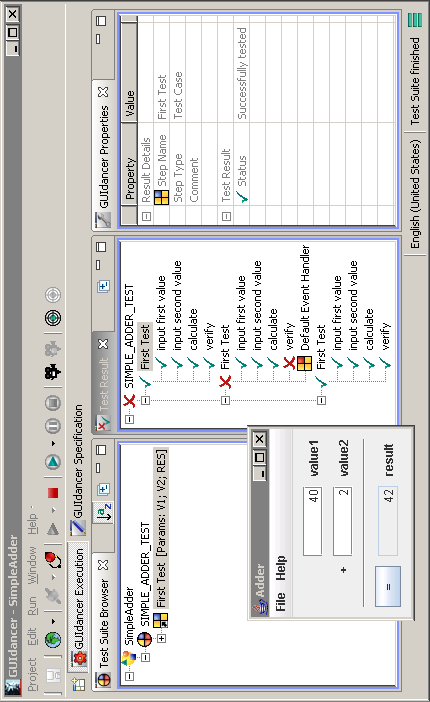
\includegraphics{Introduction/PS/Execution}
\caption{Example \gdsuite{}}
\label{Testshot}
\end{figure}



 \end{enumerate}
